% Exercise illustration: Compute the pressure of an ideal gas in three dimensions upon a wall at $x = 0$ that attracts molecules at large distance and repels them at smaller distance. Let the force be given by the potential $U(x) = -A \, e^{-\alpha x} + B \, e^{-2 \alpha x}$, with $A,B > 0$.

\documentclass[tikz,border=0 1]{standalone}

\usetikzlibrary{patterns,decorations.markings,backgrounds}

\begin{document}
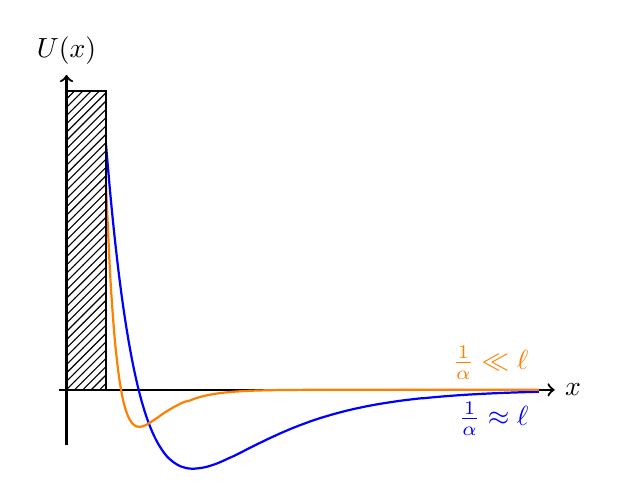
\begin{tikzpicture}[thick]

  % Axes
  \def\xmin{-0.1}\def\xmax{6}
  \def\ymin{-0.7}\def\ymax{4}
  \draw[->] (\xmin,0) -- (\xmax+0.2,0) node[right] {$x$};
  \draw[->] (0,\ymin) -- (0,\ymax) node[above] {$U(x)$};

  % Potential
  \def\wall{0.5}
  \def\U{-\A*e^(-\a*\x) + \B*e^(-2*\a*\x)}
  \def\A{10}\def\B{25}\def\a{1}
  \draw[domain=\wall:\xmax,smooth,samples=100,blue] plot ({\x},{\U}) node [below left] {$\frac{1}{\alpha} \approx \ell$};
  \def\A{15}\def\B{120}\def\a{3}
  \draw[domain=\wall:\xmax,smooth,samples=100,orange] plot ({\x},{\U}) node [above left] {$\frac{1}{\alpha} \ll \ell$};

  % Wall
  \draw[pattern=north east lines] (0,0) rectangle (\wall,\ymax-0.2);

\end{tikzpicture}
\end{document}